\documentclass{llncs}

\newif\ifpdf
\ifx\pdfoutput\undefined
   \pdffalse     % no PDFLaTeX
\else
  \pdfoutput=1  % PDFLaTeX
   \pdftrue
\fi

\usepackage{alltt}

\ifpdf
\usepackage[pdftex,bookmarks=false,
            plainpages=false,naturalnames=true,
            colorlinks=true,pdfstartview=FitV,
            linkcolor=blue,citecolor=blue,urlcolor=blue]{hyperref}
\else
\usepackage[dvips]{hyperref}
\fi

\ifpdf
\usepackage[pdftex]{graphicx}
\else
\usepackage{graphicx}
\fi

\begin{document}

\pagestyle{empty}

\mainmatter

% --- Author Metadata here ---
%\conferenceinfo{CASSS}{Marseille, France}
%\copyrightyear{2004}
% --- End of Metadata ---

\title{ESC/Java2: Uniting ESC/Java and JML}
\subtitle{Progress and issues in building and using ESC/Java2
and a report on a case study involving the use of ESC/Java2
to verify portions of an Internet voting tally system}

\author{David R.~Cok\inst{1} \and Joseph R.~Kiniry\inst{2}}
\authorrunning{David R.~Cok \and Joseph R.~Kiniry}
\institute{457 Hillside Avenue\\
  Rochester, NY 14610, USA\\
  \email{cok@frontiernet.net}
  \and
  Security of Systems Group,
  Computing Science Department\\
  University of Nijmegen,
  Toernooiveld 1\\
  6525 ED Nijmegen, The Netherlands\\
  \email{kiniry@cs.kun.nl}}
\date{May 2004}

\maketitle

\newcommand{\myhref}[2]{\ifpdf\href{#1}{#2}\else\htmladdnormallinkfoot{#2}{#1}\fi}

\begin{abstract}
  The ESC/Java tool was a lauded advance in effective static checking
  of realistic Java programs, but has become out-of-date with respect
  to Java and the Java Modeling Language (JML).  The ESC/Java2
  project, whose progress is described in this paper, builds on the
  final release of ESC/Java from DEC/SRC in several ways.  It parses
  all of JML, thus can be used with the growing body of JML-annotated
  Java code; it has additional static checking capabilities; and it
  has been designed, constructed, and documented in such a way as to
  improve the tool's usability to both users and researchers.  It is
  intended that ESC/Java2 be used for further research in, and
  larger-scale case studies of, annotation and verification, and for
  studies in programmer productivity that may result from its
  integration with other tools that work with JML and Java.  The
  initial results of the first major use of ESC/Java2, that of the
  verification of parts of the tally subsystem of the Dutch Internet
  voting system are presented as well.
\end{abstract}

%% \category{D.2.4}{Software Engineering}
%%                 {Software/Program Verification}
%%                 [Formal methods, Programming by Contract]
%% \category{F.3.1}{Logics and Meanings of Programs}
%%                 {Specifying and Verifying and Reasoning about Programs}
%%                 [assertions, invariants, logics of programs,
%%                 pre- and post-conditions, specification techniques]

%% \keywords{JML, ESC/Java, ESC/Java2, static analysis, verification,
%%           annotation languages, program specification} 

% to discuss: specs for JCE packages

\section{Introduction}

The ESC/Java tool developed at DEC/SRC was a pioneering tool in the
application of static program analysis and verification technology to
annotated Java programs~\cite{Flanagan-etal02}.  The tool and its
built-in prover operated automatically with reasonable performance and
needed only program annotations against which to check a program's
source code.  The annotations needed were easily read, written and
understood by those familiar with Java and were partially consistent
with the syntax and semantics of the separate Java Modeling Language
(JML) project~\cite{jmlpapers,Leavens-etal00}.  Consequently, the
original ESC/Java (hereafter called DEC/SRC ESC/Java) was a research
success and was also successfully used by other groups for a variety
of case studies (e.g.,~\cite{Hub03,HOP04}).

Its long-term utility, however, was lessened by a number of factors.
First, as companies were bought and sold and research groups
disbanded, there was no continuing development or support of DEC/SRC
ESC/Java, making it less useful as time went by.  As a result of these
marketplace changes, the tool was untouched for over two years and its
source code was not available.

The problem of lack of support was further compounded because its
match to JML was not complete and JML continued to evolve as research
on the needs of annotations for program checking advanced.  This
unavoidable divergence of specification languages made writing,
verifying, and maintaining specifications of non-trivial APIs
troublesome (as discussed in Section~\ref{sec:usage-exper-date}).

Additionally, JML has grown significantly in popularity.  A number of
tools have been developed that use JML, representing the work of
several
groups~\cite{jmlpapers,Burdy-etal03,Leavens-etal00,NimmerErnst01,Bogor03}.
Thus, many new research tools worked well with ``modern'' JML, but
DEC/SRC ESC/Java did not.

Finally, some of the deficiencies of the annotation language used by
DEC/SRC ESC/Java reduced the overall usability of the tool.  For
example, frame conditions were not checked, but errors in frame
conditions could cause the prover to reach incorrect conclusions.
Also, the annotation language lacked the ability to use methods in
annotations, limiting the annotations to statements only about
low-level representations.

The initial positive experience of DEC/SRC ESC/Java inspired a vision
for an industrial-strength tool that would also be useful for ongoing
research in annotation and verification.  Thus, when the source code
for DEC/SRC ESC/Java was made available, the authors of this paper
began the ESC/Java2 project.

This effort has the following goals:
(1) to make the source consistent with the current version of Java;
(2) to fully parse the current version of JML and Java;
(3) to check as much of the JML annotation language as feasible,
consistent with the original engineering goals of DEC/SRC ESC/Java
(usability at the expense of full completeness and soundness);
(4) to package the tool in a way that enables easy application in a
variety of environments, consistent with the licensing provisions of
the source code release; and
(5) as a long-term goal, and if appropriate, to update the related
tools that use the same code base (Calvin, RCC, and
Houdini~\cite{flanagan01houdini}) and to integrate with other
JML-based tools.  This integration will enable testing the tool's
utility in improving programmer productivity on significant bodies of
Java source; the tool will also serve as a basis for research in
unexplored aspects of annotation and static program analysis.
  
We have released over seven alpha versions of ESC/Java2.  The latest
version is available on the \htmladdnormallinkfoot{web}
{http://www.niii.kun.nl/ita/sos/projects/escframe.html} and we
encourage experimentation and feedback.  The source code is available
(and additional contributors are welcome) and is subject to fairly
open licensing provisions.  The discussion below of various features
of JML and ESC/Java2 is necessarily brief; more detail is available in
the implementation notes that are part of an ESC/Java2 release.

The subsequent sections will discuss the principal changes made to
DEC/SRC ESC/Java in creating ESC/Java, the extensions to static
checking, the backwards incompatibilities introduced, unresolved
semantic issues in JML, and the direction of the ongoing work in this
project.  Also discussed are ESC/Java2's first serious use: the
verification of portions of the tally subsystem of the Dutch Internet
voting system.

Appendices list the details of the enhancements to DEC/SRC ESC/Java
and those features of JML that are not yet implemented in ESC/Java2.
We fully acknowledge that the on-going work described here builds on
two substantial efforts: the definition of the Java Modeling Language
and the production of DEC/SRC ESC/Java and the Simplify prover in the
first place.

\section{Changes to DEC/SRC ESC/Java}

Creating ESC/Java2 required a number of changes to the DEC/SRC
ESC/Java tool.  Here we present the most significant of these.

\subsection{Java 1.4}

The original work was performed from 1998 to 2000, and Java has
evolved since then.\footnote{In fact, Java 1.5 went beta recently.  No
  work has begun on parsing or statically checking Java 1.5 code.
  Interested parties are welcome to contact the authors with regard to
  this topic.}  The addition required by Java 1.4 is support for the
Java {\tt assert} statement.

JML itself contains a similar assert statement.  Hence, the user may
make a choice between two behaviors.  A Java assert statement may be
interpreted simply as another language feature whose behavior is to be
modeled.  The corresponding behavior is to raise an
\texttt{AssertionError} exception under appropriate circumstances.
Alternatively, a Java assert statement may be interpreted as a JML
assert statement.  In this case, the static checker will report a
warning if the assertion predicate cannot be established.  Both
alternatives are available through user-specified options.

\subsection{Current JML}

The Java Modeling Language is a research project in itself; hence the
JML syntax and semantics are evolving and are somewhat of a moving
target (and there is as yet no complete reference manual).  However,
the core language is reasonably stable.  The following are key
additions that have been implemented; other changes that relate
primarily to parsing and JML updates are listed in the Appendix:

\setlength{\partopsep}{0in}\setlength{\parskip}{0in}\setlength{\itemsep}{0in}\setlength{\topsep}{0in}
\begin{itemize}
\setlength{\partopsep}{0in}\setlength{\parskip}{0in}\setlength{\itemsep}{0in}\setlength{\topsep}{0in}
\item inheritance of annotations and of \texttt{non\_null} modifiers
  that is consistent with the behavioral inheritance of JML;
\item support for datagroups and \texttt{in} and \texttt{maps}
  clauses, which provides a sound framework for reasoning about the
  combination of frame conditions and subtyping;
\item model import statements and model fields, routines, and types,
  which allow abstraction and modularity in writing specifications;
\item enlarging the use and correcting the handling of scope of ghost
  fields, so that the syntactic behavior of annotation fields matches
  that of Java and other JML tools.
\end{itemize}
In addition, virtually all of the differences between JML and DEC/SRC
ESC/Java noted in the JML Reference Manual have been resolved.

\subsection{New verification checks}
Though all of JML is parsed, not all of it is currently checked.
Static checking of the following features has been added to that
performed by DEC/SRC ESC/Java.  The space available in this paper
permits only a summary of the embedding of the above into the
underlying ESC/Java logic.\footnote{Subsequent papers are planned that
  will describe these embeddings in more detail.}

\paragraph*{The constraint and initially clauses}
These two clauses are variations on the more common \texttt{invariant}
clause.  They apply to the whole class.  A constraint states a
condition that must hold between the pre-state and the post-state of
every method of a class.  For example,
\begin{center}
\texttt{constraint maxSize == \char'134 old(maxSize); }
\end{center}
states that \texttt{maxSize} is not changed by any method of the
class.  It is implemented by adding the predicate as a postcondition
of every (non-helper) method in the type (and its derived types).

Similarly, \texttt{initially} states a condition that must hold of
every object after construction.  It is implemented by adding its
predicate as a postcondition of every (non-helper) constructor of the
type (but not of its derived types).

\paragraph*{The \texttt{\char'134 not\_modified} expression}
The \texttt{not\_modified} construct is a way of saying, within a
postcondition, that a particular expression has the same value in the
pre-state and the post-state.  That is,
\begin{center}
\texttt{\char'134 not\_modified(x+y) $\equiv$ ( (x+y) == \char'134 old(x+y) )  }.
\end{center}
Uses of the expression in postconditions are expanded inline according
to this definition.

\paragraph*{Checking of datagroups and frame conditions}
JML contains syntax to define 
datagroups~\cite{Leino-Poetzsch-Heffter-Zhou02}.  With datagroups, the items in
an \texttt{assignable} clause may represent sets of program locations,
and those sets may be extended by subtypes.  Each
specification case of a routine may be guarded by a
precondition and may specify the set of store locations that may be
assigned to.

There are a number of cases to be considered in a full implementation.
We will discuss just one here: an assignment statement that has a
left-hand side of \textit{expr.field}.  For this to be a legal
assignment with respect to the specifications, either (a) the
\textit{expr} must evaluate to an object that has been allocated since
the beginning of the execution of the method, or (b) it must be the
case that for every specification case of the method containing the assignment
for which the precondition is true (in the pre-state) there is at
least one store location in the list of assignable locations that
matches \textit{expr.field}.  To match, the field names must be the
same and the \textit{expr} values must evaluate to the same object.
The matching is complicated by the variety of syntax (e.g.
\textit{expr}\texttt{.*} matches any field of \textit{expr}) and by
the fact that a given field designation may have an accompanying
datagroup and the match may be to any element of the datagroup.

The most substantial complication is that datagroups may be
recursively defined and thus may have unbounded size.  For example,
consider the datagroup of all of the `next' fields of a linked list.
ESC/Java2 currently deals with this by unrolling the recursion to a
fixed depth; since in ESC/Java loops are also unrolled to a fixed
number of iterations, this solution handles common cases of iterating
over recursive structures.

\paragraph*{Annotations containing routine calls and dynamic allocations}
JML, but not DEC/SRC ESC/Java, allows pure method calls to be used in
annotations.  This allows both a degree of abstraction and more
readable and writable specifications.  ESC/Java2 supports the JML
syntax and also performs some static checking.  The underlying prover,
Simplify, does support function definitions and reasoning with
functions.  But, as is the rule in first-order provers, the result of
a function depends only on its arguments and not on hidden arguments
or on global structures referenced by the arguments.  Consequently
there is a mismatch between the concept of a method in Java and the
concept of a function in the prover.  However, a moderate degree of
checking can be performed without resorting to a full state-based
translation and logic if we (a) identify some methods as functions,
where possible, (b) include the current state of the heap as an
additional uninterpreted parameter, and (c) incorporate the
specifications of the called method as additional axioms.

Dynamic allocations of objects using constructors can be recast as
method calls and treated as described above.  Dynamic allocations of
arrays can be translated into first-order logic as functions without
difficulty.

\paragraph*{model fields and represents clauses}
The combination of \texttt{represents} clauses and model fields
provides a substantial benefit in abstraction, especially since the
representations may be provided by a subtype \cite{Cheon-etal03}.
Simple representations can be implemented in ESC/Java2 by inlining the
representation wherever the model field is used in an annotation.
However, that proves not to be workable in larger systems.  Instead,
we translate instances of model fields as functions of the object that
owns them and the global state.  This allows a useful degree of
reasoning when combined with the class invariants that describe the
behavior of the model fields.

\subsection{Backwards incompatibilities}
The DEC/SRC ESC/Java specification language and JML arose separately;
there was some initial but incomplete work to unify the two.  The
ESC/Java2 project intends to have the tool reflect JML as precisely as
reasonable.  In some cases, discussion about differences resulted in
changes to JML.  In a few cases, some backwards incompatibilities in
DEC/SRC ESC/Java were introduced.  The principal incompatibilities are
these:
\setlength{\partopsep}{0in}\setlength{\parskip}{0in}\setlength{\itemsep}{0in}\setlength{\topsep}{0in}
\begin{itemize}
\setlength{\partopsep}{0in}\setlength{\parskip}{0in}\setlength{\itemsep}{0in}\setlength{\topsep}{0in}
\item The semantics of inheritance of specification clauses and of
  \texttt{non\_null} modifiers was modified to match that defined by
  JML, since the work on JML resulted in an interpretation consistent
  with behavioral subtyping.  This also changed the usage and
  semantics of the \texttt{also} keyword.
\item The specification \texttt{modifies \char'134 everything} is now
  the default frame axiom.
\item The syntax and semantics of \texttt{initially},
  \texttt{readable\_if} and \texttt{monitored\_by} have changed.
\item ESC/Java2 forbids bodies of (non-model) routines to be present
  in non-Java specification files.
\end{itemize}

\section{Unresolved semantic issues}
%%TODO - Gary suggest concentrating on the important issues.

The work on ESC/Java2 has been useful in exposing and resolving
semantic issues in JML.  Since ESC/Java2 is built on a different
source code base than other JML tools, differences of interpretation
in both syntax and semantics arise on occasion.  These are generally
resolved and documented via mailing list discussions\footnote{See
  \texttt{jmlspecs-interest@lists.sourceforge.net},\\
  \texttt{jmlspecs-developers@lists.sourceforge.net}, and \\
  \texttt{jmlspecs-escjava@lists.sourceforge.net} or the corresponding
  archives at \url{http://sourceforge.net/projects/jmlspecs}} by
interested parties.  There are, however, still unresolved issues, most
of which are the subject of ongoing research.
\setlength{\partopsep}{0in}\setlength{\parskip}{0in}\setlength{\itemsep}{0in}\setlength{\topsep}{0in}
\begin{itemize}
\setlength{\partopsep}{0in}\setlength{\parskip}{0in}\setlength{\itemsep}{0in}\setlength{\topsep}{0in}
%% There are "however" in 5 of the 7 sections below. -JRK  TODO
\item \textit{pure routines}: It is convenient and modular to use
  model and Java methods within annotations.  The semantics of such
  use is clearer and simpler if such routines are {\em pure}, that is,
  they do not have side-effects.  This is important when evaluating
  annotations during execution, since the checking of specifications
  should not affect the operation of the program being checked.
  Side-effects also complicate static reasoning.  However, some
  side-effects are always present, such as changes to the stack or
  heap or external effects such as the passage of time.  Some are
  often overlooked but can be consequential, such as locking a
  monitor.  Others the programmer may see as innocuous, benevolent
  side-effects, such as maintaining a private cached value or logging
  debugging information in an output file.  An interpretation of the
  combination of purity and benevolent (or ignorable) side-effects
  that is suitable for both static and run-time checking and is
  convenient and intuitive for users is not yet available. (See also
  the discussion of purity checking in~\cite{Leavens-etal03a}.)
\item \textit{exceptions in pure expressions}: The expressions used in
  annotations must not have side-effects, but they may still throw
  exceptions.  In that case the result is ill-defined.  A semantics
  that is suitable for both run-time checking and static verification
  needs to be established.
\item \textit{initialization}: The authors are not aware of any
  published work on specifying the initialization of classes and
  objects in the context of JML; initial work formalizing
  \texttt{\char'134 not\_initialized} was only recently completed for
  the Loop tool.  This task includes providing syntax and semantics
  for Java initialization blocks, JML's \texttt{initializer} and
  \texttt{static\_initializer} keywords, and formalizing the rules
  about order of initialization of classes and object fields in Java.
\item \textit{datagroups}: The \texttt{in} and \texttt{maps} clauses
  and the datagroup syntax are designed to allow the specification of
  frame conditions in a sound way that is extensible by derived
  classes.  We do not yet have experience with the interaction among
  datagroups, the syntax for designating store locations, and either
  reasoning about recursive data structures or checking them at
  run-time.
\item \textit{unbounded arithmetic}: Chalin~\cite{Chalin03} has
  proposed syntax and semantics to enable specifiers to utilize
  unbounded arithmetic in a safe way within annotations.  Tool support
  and experience with these concepts is in progress.  Axioms and proof
  procedures will be needed to support this work in static checkers.
\end{itemize}
There are other outstanding but less significant issues concerning
helper annotations, model programs and the \texttt{weakly},
\texttt{hence\_by}, \texttt{measured\_by}, \texttt{accessible} and
\texttt{callable} clauses.

\section{Usage experience to date}
\label{sec:usage-exper-date}
The SoS group at the University of Nijmegen, along with other members
of the \htmladdnormallinkfoot{European VerifiCard
  Project}{http://www.verificard.org/}, has used DEC/SRC ESC/Java for
several projects.  For example, Hubbers, Oostdijk, and Poll have
performed verifications of Smart Card applets using several tools,
including DEC/SRC ESC/Java~\cite{HOP04}.  Hubbers has also taken
initial steps integrating several JML-based tools~\cite{Hub03}.

These and other VerifiCard projects relied upon the specifications of
the Java Card 2.1.1 API written and verified by Poll, Meijer, and
others~\cite{MeijerPoll01}.  This specification originally came in two
forms: one ``heavyweight'' specification that used JML models,
heavyweight contract specifications, and refinements, and another
``lightweight'' specification that was meant to be used with DEC/SRC
ESC/Java and other verification tools like Jack, Krakatoa, and the
Loop tool~\cite{BergJ01,BurdyRequet02,MarchePaulinMohringUrbain04}.

Writing, verifying, and maintaining these two specifications was a
troublesome experience.  Because of limitations of various tools which
depended upon the specifications, several alternate forms of
specifications were required.  Additionally, it was sometimes the case
that the alternate forms were neither equivalent nor had obvious
logical relationships between them.

This experience was one of the motivators for the SoS group's support
of this work on ESC/Java2.  Now that multiple tools are available that
fully cover the JML language, the incidence of specification reuse is
rising and painful maintenance issues are becoming a thing of the
past.  As a result, early evidence for the success of this transition
is beginning to appear.

\subsection{Transitional Verifications}

First, the specifications of a small case
study~\cite{BreunesseJacobsBerg02} were updated and re-verified by one
of this paper's authors (Kiniry) using ESC/Java2.  The original work
depended upon ``light\-weight'' JML specifications of core Java Card
classes and the verification was performed with DEC/SRC ESC/Java and
the Loop tool.  The re-verification effort used the full
``heavyweight'' Java and Java Card specifications and was accomplished
in a single afternoon.

Second, several members of the SoS group are contributing to updating
the ``heavyweight'' JML specifications of the Java Card API.  As a
part of this work, the Gemplus Electronic Purse case study, which has
been verified partially with DEC/SRC ESC/Java~\cite{CatanoHuisman02}
and partially with the Loop tool~\cite{BreunesseJacobsBerg02}, is
being re-verified completely with ESC/Java2 using ``heavyweight''
specifications.

Finally, recent attempts at verifying highly complex Java code
examples written by Jan Bergstra and originally used as stress-tests
for the Loop tool have been encouraging.  Methods that originally took
a significant amount of interactive effort to verify in PVS are now
automatically verified in ESC/Java2, much to the surprise of some of
the Loop tool authors.  This work has caused some re-evaluation of the
balance between interactive and automated theorem proving in the SoS
group.

\subsection{Verification of an Electronic Voting Subsystem}

The first major partial verification using ESC/Java2 took place in
early 2004.

The Dutch Parliament decided in 2003 to construct an Internet-based
remote voting system for use by Dutch expatriates.  The SoS group was
part of an expert review panel for the system and also performed a
black-box network and system security evaluation of this system in
late 2003.  A recommendation of the panel was that a third party
should construct a redundant tally system.  Such a second system would
ensure a double-check of the election count with an independent
system.  It was also thought that such an external implementation
would provide some third-party review of the original work, as the new
implementation would depend entirely upon system design documentation
and data artifacts (e.g. candidate and vote files); no source code
would be shared, or even seen, by the team implementing the redundant
system.

The SoS group bid on the construction of this new system, emphasizing
the fact that they would use formal methods (specifically, JML and
ESC/Java2) to specify, test, and verify the tally system.  The bid was
successful, and as a result the SoS group was contracted to write the
tally system.

The most challenging aspect of the contract was \emph{not} the use of
formal methods.  Instead, it was the strict \emph{time requirements}
of the contract, as the system was to be used in the upcoming European
elections.  In particular, the SoS group was asked to construct the
vote counting system (henceforth called the \textsc{KOA} system) in
approximately \emph{four weeks}, with only three developers.

\subsubsection{Development Methodology}

To approach this problem, the three developers (Dr.~Engelbert Hubbers,
Dr.~Martijn Oostdijk, and the second author) partitioned the system
into three subcomponents: file I/O, graphical I/O, and core
data structures and algorithms.  It was decided that, due to the
challenges inherent in full system verification and the restricted
time alloted to the project, while all subsystems would be annotated
with JML, only the third ``core'' subsystem (Dr.~Kiniry's
responsibility) would be fully elaborated in specification.

Additionally, ESC/Java2 would only be used on the core subsystem.  In
the alloted time a ``best-effort'' verification would be attempted, in
addition to all other standard software engineering practices.  This
approach is a standard strategy for lightweight use of formal
methods~\cite{ClarkeWing96}.

\begin{table}[htbp]
  \caption{KOA System Summary}
  \label{tab:KOA_System_Summary}
  \begin{center}
    \begin{tabular}{|l|ccc|}
      \hline
      \quad     & \textbf{File I/O} & \textbf{Graphical I/O} & \textbf{Core} \\
      \hline
       classes & 8                 & 13                     & 6             \\
       methods & 154               & 200                    & 83            \\
      NCSS      & 837               & 1,599                  & 395           \\
      Specs     & 446               & 172                    & 529           \\
      Specs:NCSS & 1:2              & 1:10                   & 5:4           \\
      \hline
    \end{tabular}
  \end{center}
\end{table}

Table~\ref{tab:KOA_System_Summary} summarizes the size, complexity,
and specification coverage of the three subsystems, as measured with
the JavaNCSS tool version 20.40 during the week of 24 May, 2004.
Assertions were counted by simply counting the number of uses of
appropriate core specification keywords (requires, ensures, invariant,
non\_null, in, set, and modifies).

\subsubsection{Specification Coverage and Methodology}

Unsurprisingly, the GUI portion of KOA is the largest subsystem with
the lightest specification coverage with approximately 1 annotation
for every 10 lines of code.  The focus of the GUI subsystem
specification is a finite state machine that represents the state of
the GUI.  The state of the KOA application is tightly coupled to this
GUI state machine as the vote courting process is highly serialized.

\begin{figure}[htbp]
  \begin{center}
    \ifpdf
    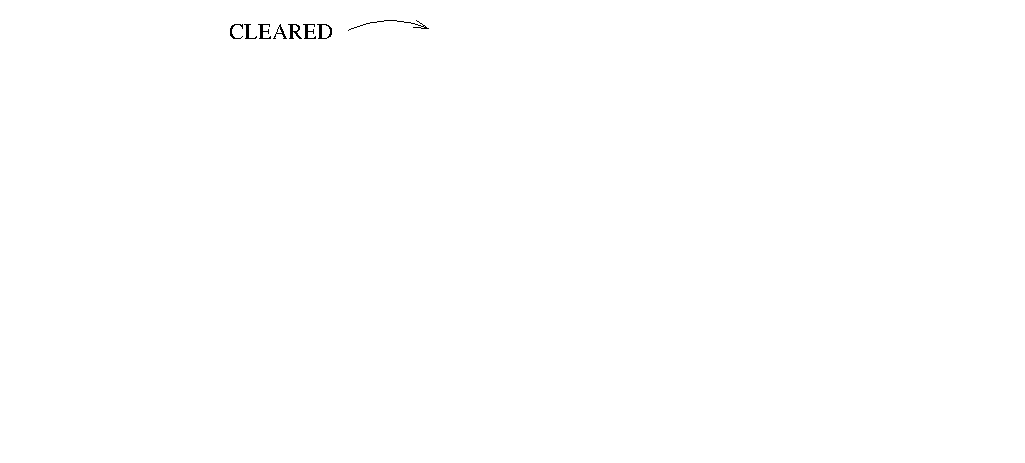
\includegraphics[width=80mm]{koa_state_diagram}
    \else
    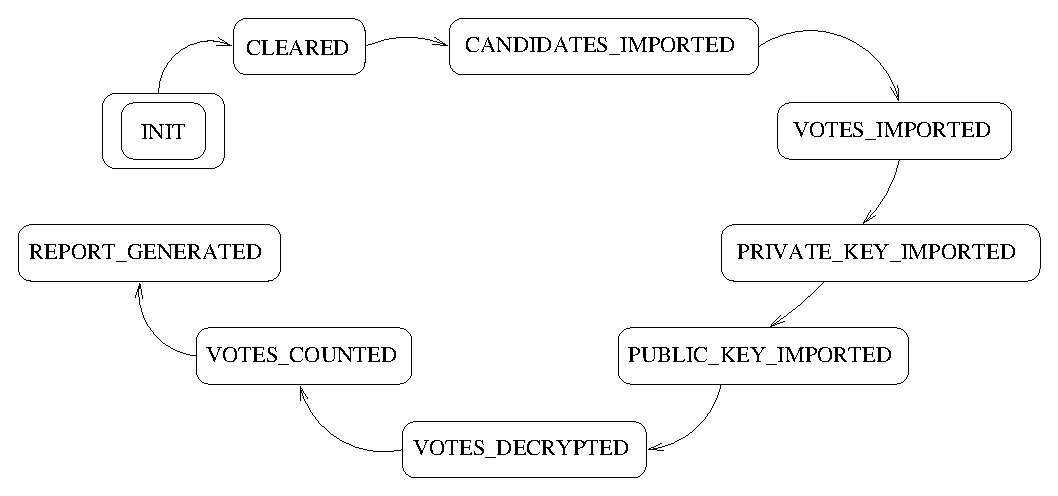
\includegraphics[width=80mm]{koa_state_diagram.eps}
    \fi
    \caption{KOA State Diagram}
    \label{fig:KOA_State_Diagram}
  \end{center}
\end{figure}
Figure~\ref{fig:KOA_State_Diagram} contains a diagram that summarizes
this state machine.  The state of the system is represented in a
(spec\_public) field ``\texttt{state}'' of the main class of the
application.  The state machine is formally modeled using the standard
mechanisms developed in the past by the SoS
Group~\cite{Hubbers_Oostdijk_Poll:2003sec}.

The file I/O subsystem exhibits better specification coverage, much of
which focuses on contracts to ensure that data-structures in the core
subsystem are properly constructed according to the contents of input
files.

The core subsystem understandably has the highest specification
coverage, at over one line of specification for every line of code.

The verification of the key properties of the system, particularly the
property of having a correct tally of votes, are directly tied to the
overall state of the system using invariants of the form
\begin{alltt}
     invariant (state >= <STATE>) ==> (state-field != null);
\end{alltt}
Such an invariant says that, if the state of the system is at least
\texttt{<STATE>}, then the appropriate representation for that state,
captured in the \texttt{state-field}'s datatype is well-formed.  This
is a strong claim because if \texttt{state-field} is non-null, then
not only is it initialized, but all of its invariants hold.

At this time, verification coverage of the core subsystem is good, but
not 100\%.  Approximately 10\% of the core methods (8 methods) are
unverified due to issues with ESC/Java's Simplify theorem prover
(either the prover does not terminate or terminates abnormally).
Another 31\% of the core methods (26 methods) have postconditions that
cannot be verified, typically due to completeness issues discussed
above, and 12\% of the methods (10 methods) fail to verify due to
invariant issues, most of which are due to suspected inconsistencies
in the specifications of the core Java class libraries or JML model
classes.  The remaining 47\% (39 methods) of the core verifies
completely.

Since 100\% verification coverage was not possible in the timeframe of
the project, and to ensure the KOA application is of the highest
quality level possible, a large number unit tests were generated with
the \emph{jmlunit} tool for all core classes.  A total of nearly 8,000
unit tests were generated, focusing on key values of the various
datatypes and their dependent base types.  These tests cover 100\% of
the core code and are 100\% successful.

\subsubsection{Impressions of ESC/Java2}

ESC/Java2 made a very positive impression on the KOA developers.  Its
increased capabilities as compared to DEC/SRC ESC/Java, particularly
with regards to handling the full JML language, the ability to reason
with models and specifications with pure methods, are very impressive.
And, while the tool is still classified as an ``alpha'' release, we
found it to be quite robust (perhaps unsurprising given its history,
the use of JML and ESC/Java2 in and on its own source code, and the
fact that it is passed through seven alpha releases thus far).  But
there are still a number of issues with ESC/Java2 and JML that were
highlighted by the KOA verification effort.

The primary issues that arose include:
\begin{itemize}
\item \emph{String semantics in ESC/Java2 are incomplete.}  In
  particular, one cannot reason effectively about String concatenation
  or equality.  While Java Strings are certainly a non-trivial type,
  the are effectively a pseudo-base type because of their prolific
  application.  Thus, it is vital that this issue is addressed as soon
  as possible.
\item \emph{Issues with reasoning about ``representation-less'' model
    variables.}  If a class declares a model variable but provides no
  statement about how that model relates to the implementation of the
  class (using a \texttt{represents} clause or similar), then
  ESC/Java2 cannot verify assertions that use the model.  We believe
  that a representation-less model variable is equivalent to a ghost
  variable since it is being used as a specification-only variable in
  an API spec.  Thus, by replacing problematic model variables with
  ghost variables in API specifications we can successfully perform
  verifications using the APIs.  This problem indicates either a
  problem with the design and/or use of model variables in JML, or an
  implementation issue with ESC/Java2.
\item \emph{Inconsistencies and ambiguities in the specification of
    core APIs, particularly classes in the \texttt{java.lang} and
    \texttt{java.util} packages and JML model classes.}  This is the
  first large-scale verification effort using ``full'' JML
  specifications of the core JDK.  These ``full'' specifications are
  much more complete and complex than those that were used with
  DEC/SRC ESC/Java.  As these core specifications have never been
  formally analyzed for consistency or completeness, it is not
  surprising that the KOA verification effort had problems with their
  use.  It is expected that over time, with more use by a range of
  JML-compatible tools the core specifications will become more
  consistent and complete to the benefit of all JML tool users.
\item \emph{Completeness issues with first-order predicates.}
  First-order predicates are expressed with the \texttt{forall} and
  \texttt{exists} constructs in JML.  Only some of these predicates
  can be used and/or verified in JML-based tools, including ESC/Java2.
  Unfortunately, many of the most interesting invariants in
  non-trivial systems can only be expressed using such constructs.
  Thus, more focus needs to be put on understanding and reasoning
  about such assertions.
\item \emph{Aliasing issues and specification convenience constructs
    for such.}  As usual, reasoning about reference types and avoiding
  aliasing was one of the key issues in verifying the KOA application.
  For example, it was frequently the case that we wished to say that a
  set of references where unique (that is, they were pairwise
  unequal).  The only way to state this in JML today is quite
  cumbersome, thus the introduction of a new specification construct
  for such seems warranted.
\end{itemize}

% JML test runs: 18/19 (meaningful/total)
% JML test runs: 35/6716 (meaningful/total)
% JML test runs: 20/37 (meaningful/total)
% JML test runs: 36/64 (meaningful/total)
% JML test runs: 48/210 (meaningful/total)
% JML test runs: 97/776 (meaningful/total)
% (+ 19 6716 37 64 210 776)

\section{Ongoing work}
The work on ESC/Java2 is continuing on a number of fronts.

\paragraph*{Language Issues} Two obvious and related ongoing tasks are
the completion of additional features of JML, accompanied in some
cases by additional research to clarify the semantics and usability of
outstanding features of JML.  Usage of JML is now broad enough that
accompanying formal reference documentation would be valuable.  As
tools such as ESC/Java2 become more widely used, users will also
appreciate attention to performance, to the clarity of errors and
warnings, and to the overall user experience such tools provide.

\paragraph*{Case Studies} The current implementation supports the
static checking of a stable core of JML.  With this initial
implementation of frame condition checking, of model fields,
represents clauses and use of routine calls in annotations, ESC/Java2
can now be used on complex and abstract specifications of larger
bodies of software.  Consequently, there is a considerable need for
good experimental usage studies that confirm that this core of JML is
useful in annotations, and that the operation of ESC/Java2 (and
Simplify) on that core is correct and valuable.

\paragraph*{Verification Logic} The logic into which Java and JML are
embedded in both DEC/SRC ESC/Java and ESC/Java2 is, by design and
admission of the original authors, neither complete or fully sound.
This was the result of an engineering judgment in favor of performance
and usability.  Research studying expanded and larger use cases may
show whether this design decision is generally useful in practical
static checking or whether a fuller and more complicated state-based
logic is required for significant results to be obtained.

A related issue is the balance between automated and manual proof
construction.  Use of verification logics will likely be limited to
narrow specialties as long as proof construction is a major component
of the overall programming task.  Thus, automation is essential,
though it is expected that full automation is infeasible.  The degree
of automation achievable will continue to be a research question.
However, we believe that broad adoption of automated tools for program
checking will require that users only need interact at high levels of
proof construction.

\paragraph*{User Feedback} The purpose of using theorem provers for
static analysis, runtime assertion checking, or model checking is to
find errors and thereby improve the correctness of the resulting
software.  Thus, the orientation of a tool must be towards effectively
finding \emph{and interpreting} examples of incorrect behavior.  A
complaint (e.g.,~\cite{GroceVisser03}) in using such technologies is
that it is difficult to determine a root cause from the counterexample
information provided by the tool, whether it is a failed proof or an
invalid test or execution history.  The DEC/SRC ESC/Java project
implemented some work towards appropriately pruning and interpreting
counterexample and trace information, but there remains room for
improvement.

\paragraph*{Tool Integration} Finally, though not part of this specific
project, an integration of tools that support JML would be beneficial
for programmer productivity.  A productive programmer's working
environment for a large-scale project that uses these tools would need
the them to be integrated in a way that they seamlessly communicate
with one another.  A programmer using the tools would naturally move
among the various tasks of designing, writing, testing, annotating,
verifying and debugging, all the while reading, writing and checking
specifications.  Design, specifications and code might all be built up
incrementally.  Thus, the tools would need to be integrated in a way
that allows efficient and iterative behavior.

\section{Conclusion}

%% I find this first paragraph, and actually the whole of the
%% conclusion a bit odd and weak.  Perhaps some lead in using Hoare03
%% would strengthen the discussion?  In case you have not yet read
%% that paper David, Tony has stated that a fully verifying compiler
%% should be one of the premire challenges of computer science for
%% the 21st century, and cites ESC/Java as the nearest approximation
%% to this goal.  I do not believe that he has yet seen our work
%% on ESC/Java2, and will be very encouraged and excited by it. -JRK - TODO

Because this work on implementing ESC/Java2 and evaluating its use is
in progress, a set of data-driven conclusions is premature.  Instead,
let us posit a hypothesis in the form of a vision.

One can observe this work in tool creation and evaluation from a
number of perspectives.  Certainly such work creates working
prototypes that test in practice theories of programming and
specification language semantics.  It also exercises and validates
ideas in automated logical reasoning.  We prefer to use the viewpoint
of programming productivity, particularly given the industrial working
environment of the first author.  In that context we observe the
existence and general use across multiple research groups of the
combination of various tools that support using JML with Java
programs; this suggests to us that the syntax and semantics of the
core of JML are sufficiently useful and natural to provide a basis for
future wider use.  With respect to logical reasoning, a useful degree
of automation is achievable in at least some aspects of static
checking tasks; removing the details of proof construction from a
programmer's tasks is essential to larger scale acceptance of such
tools.

However, the surrounding issues are as relevant to programmer
acceptance and productivity.  Tools must have intuitive and
unsurprising behavior. They must be efficient in elapsed run-time, but
also in the time needed to interpret and act upon the results.  They
must integrate well with other tools of the same family and with the
commonly used programmer's working environments.

%%TODO - Gary doesn't like the second part of the following paragraph

There is progress on enough of the above vectors that one might well
be optimistic about the eventual success of the enterprise as a whole.
After all, the goal need not be fully automated verification of an
arbitrary computer program.  Reflect that a computer-produced proof of
a mathematical conjecture that cannot be understood at least in its
broad outlines by mathematicians leaves those mathematicians
unsatisfied and unsettled with respect to the result.  Similarly, we
expect that ``verifications'' of programs whose overall design is
incomprehensible to readers of the program (not to mention its author)
will not engender much confidence in the result.  If programming is
writing for others and we expect that the authors could explain their
programs to their colleagues, we may well have a chance at being able
to explain those programs to a computer.

%\large\textbf{TODO:}\normalsize Perhaps discuss the fact that a
%verifying compiler might be closer than some notable computer
%scientists think~\cite{Hoare03}?  Discuss how far we think that we can
%take this application of basic logics, first-order provers, and
%related technologies.  Also reinforce the changing balance between
%automated and interactive proving, discussed in the usage experience
%section above. -JRK

%ACKNOWLEDGMENTS are optional
\section{Acknowledgments}
The authors would like to acknowledge both the work of the team that
generated DEC/SRC ESC/Java as well as Gary Leavens and collaborators
at Iowa State University who generated JML.  In addition, Leavens and
students engaged in and helped resolve syntactic and semantic issues
in JML raised by the work on ESC/Java2.  These teams provided the twin
foundations on which the current work is built.  Other research groups
that use and critique both JML and ESC/Java2 have provided a research
environment in which the work described here is useful.  Thanks are
due also to Leavens for his comments on an eaarly draft of this paper.

Joseph Kiniry is supported by the NWO Pionier research project on
Program Security and Correctness and the VerifiCard research project.

%
% The following two commands are all you need in the
% initial runs of your .tex file to
% produce the bibliography for the citations in your paper.
\bibliographystyle{abbrv}
\bibliography{abbrev,PASTE2004,CASSIS2004}
% To create the self-contained file - comment out the line above and include the
% contents of the .bbl file here
%% \begin{thebibliography}
%% \end{thebibliography}

% You must have a proper ".bib" file
%  and remember to run:
% latex bibtex latex latex
% to resolve all references
%
% ACM needs 'a single self-contained file'!
%
%APPENDICES are optional

%\balancecolumns

\appendix

\section{Principal changes in ESC/Java}
\setlength{\partopsep}{0in}\setlength{\parskip}{0in}\setlength{\itemsep}{0in}\setlength{\topsep}{0in}
\begin{itemize}
\setlength{\partopsep}{0in}\setlength{\parskip}{0in}\setlength{\itemsep}{0in}\setlength{\topsep}{0in}
\item[] \textit{Language semantics}
\item inheritance of annotations and of \texttt{non\_null}
  modifiers that is consistent with the behavioral inheritance of JML;
\item support for datagroups and \texttt{in} and \texttt{maps} clauses, which provides a sound framework for reasoning about the combination of frame conditions and subtyping;
\item model import statements and model fields, routines, and types, which allow abstraction 
and modularity in writing specifications;
\item enlarging the use and correcting the handling of scope of ghost fields, so that the syntactic behavior 
of annotation fields matches that of Java and other JML tools;
\item[]
\item[] \textit{Language parsing}
\item parsing of all of current JML, even if the constructs are
  ignored with respect to typechecking or verification;
\item support for refinement files, which allow specifications to be supplied in files separate from the source code or in the absence of source code;
\item heavyweight annotations, which allow some degree of modularity and nesting;
\item auto model import of the \texttt{org.jmlspecs.lang} package, similar to Java's auto import of \texttt{java.lang};
\item generalizing the use of \texttt{\char'134 old}, \texttt{set} statements and local ghost variables, to provide more flexibility in writing specifications;
\item introduction of the \texttt{constraint}, \texttt{represents}, \texttt{field}, \texttt{method},
\texttt{constructor}, 
\texttt{\char'134 not\_modified}, \texttt{instance}, \texttt{old}, \texttt{forall},
\texttt{pure} keywords as defined in JML; and
\item consistency in the format of annotations in order to match the language handled by other JML tools.
\item equivalence of \texttt{\char'134 TYPE} and \texttt{java.lang.Class};
\end{itemize}
In addition, virtually all of the differences between JML and DEC/SRC ESC/Java
noted in the JML Reference Manual have been resolved.

\section{Aspects of JML not yet\\implemented in ESC/Java2}

Though the core is well-supported, there are several features of JML
which are parsed and ignored, some of them experimental or not yet
endowed with a clear semantics, and some in the process of being
implemented.  For those interested in the details of JML and
ESC/Java2, the features that are currently ignored are the following:
\setlength{\partopsep}{0in}\setlength{\parskip}{0in}\setlength{\itemsep}{0in}\setlength{\topsep}{0in}
\begin{itemize}
\setlength{\partopsep}{0in}\setlength{\parskip}{0in}\setlength{\itemsep}{0in}\setlength{\topsep}{0in}
\item checking of access modifiers on annotations and of the
 \texttt{strictfp}, \texttt{volatile},
  \texttt{transient} and \texttt{weakly} modifiers;
\item the clauses \texttt{diverges}, \texttt{hence\_by},
  \texttt{code\_contract}, \texttt{when}, and \texttt{measured\_by};
\item the annotations within \texttt{implies\_that} and {\tt
    for\_example} sections;
\item some of the semantics associated with the initialization steps prior to
  construction;
\item multi-threading support beyond that already provided in DEC/SRC ESC/\-Java;
\item serialization;
\item annotations regarding space and time consumption;
\item full support of recursive \texttt{maps} declarations;
\item model programs;
\item some aspects of store-ref expressions;
\item verification of anonymous and block-level classes;
\item verification of set comprehension and some forms of quantified
  expressions;
\item implementation of \texttt{modifies \char'134 everything} within
  the body of routines.
\end{itemize}


% That's all folks!
\end{document}

